% Lim declaration from the local amsldoc.tex operator-name example.
\documentclass[border=2pt]{standalone}
\usepackage{amsmath}
\usepackage{tikz}
\DeclareMathOperator*{\Lim}{Lim}
\DeclareMathOperator*{\argmin}{arg\,min}
\begin{document}
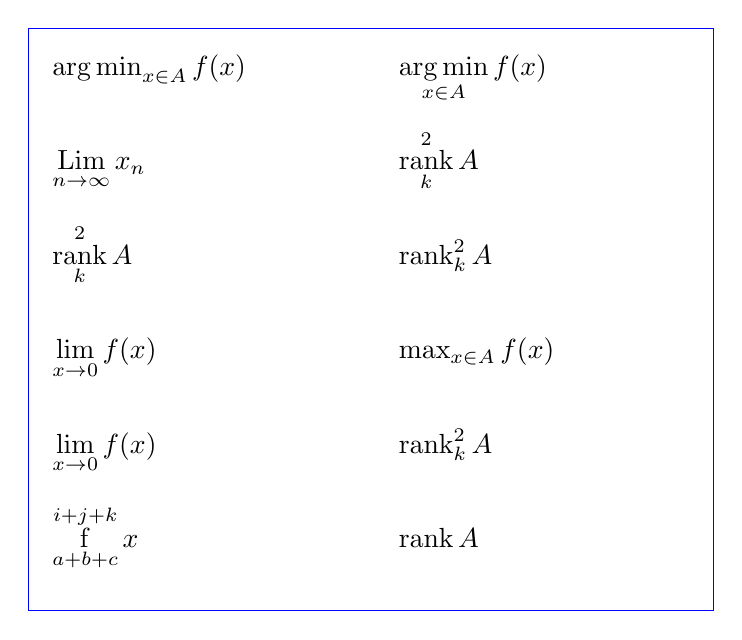
\begin{tikzpicture}
  \draw[blue] (-.3,.6) rectangle (8.4,-6.8);
  \node[anchor=base west,inner sep=0] at (0,0) {$\operatorname*{arg\,min}_{x\in A}f(x)$};
  \node[anchor=base west,inner sep=0] at (4.4,0) {$\displaystyle\argmin_{x\in A}f(x)$};
  \node[anchor=base west,inner sep=0] at (0,-1.2) {$\displaystyle\Lim_{n\to\infty}x_n$};
  \node[anchor=base west,inner sep=0] at (4.4,-1.2) {$\displaystyle\operatorname*{rank}^2_k A$};
  \node[anchor=base west,inner sep=0] at (0,-2.4) {$\operatorname*{rank}\limits^2_k A$};
  \node[anchor=base west,inner sep=0] at (4.4,-2.4) {$\displaystyle\operatorname*{rank}\nolimits^2_k A$};
  \node[anchor=base west,inner sep=0] at (0,-3.6) {$\displaystyle\lim_{x\to0}f(x)$};
  \node[anchor=base west,inner sep=0] at (4.4,-3.6) {$\max_{x\in A}f(x)$};
  \node[anchor=base west,inner sep=0] at (0,-4.8) {$\lim\limits_{x\to0}f(x)$};
  \node[anchor=base west,inner sep=0] at (4.4,-4.8) {$\displaystyle\operatorname{rank}\limits^2_k A$};
  \node[anchor=base west,inner sep=0] at (0,-6) {$\displaystyle\operatorname*{f}^{i+j+k}_{a+b+c}x$};
  \node[anchor=base west,inner sep=0] at (4.4,-6) {$\displaystyle\operatorname*{rank}^{}_{} A$};
\end{tikzpicture}
\end{document}
